\documentclass[12pt,oneside,english,palatino]{book}
\usepackage{graphicx}

\newcommand{\units}[1]{\ensuremath{[\mathrm{#1}]}}
\newcommand{\parameter}[2]{{\texttt{#1}} (#2)}
\begin{document}

\title{The ModAEM Book\\
Version 1.9.0}

\author{Vic Kelson, Ph.D. PE \\
WHPA Inc.\\
320 West 8th St.\\
Bloomington, IN 47404}

\maketitle
\tableofcontents{}

\listoffigures

\chapter{Introduction\label{cha:Introduction} }

This manual describes the results of nearly 20 years of effort (much
of it the ``on again, off again'' variety). ModAEM has been through
four major revisions, several research branches, and has been used
for countless wellhead protection models, even though most ModAEM
users never knew they were using it! This chapter is to introduces
to the history and philosophy of ModAEM. 


\subsection*{Early ModAEM}

The essential design of ModAEM was conceived during a series of long
discussions between Mark Bakker, Steve Kraemer, and myself during
a High Performance Computing Consortium workshop at EPA's Research
Triangle Park facility in 1995 (I was first introduced to the ``new''
GMS preprocessor at the same meeting). I'm not sure that Steve and
Mark remember the meeting or the design ideas, but they basically
remain intact:
\begin{itemize}
\item Logical separation of the analytic element \emph{functions} (dipoles/doublets,
wells, etc.) from analytic element \emph{applications} (wells, rivers,
inhomogeneities)
\item Implementation of efficient functions for a few very flexible analytic
element functions (at that time, only wells, dipoles of complex strength,
and ponds were anticipated)
\item Make it all parallelizable with very little effort
\item Abandon FORTRAN 77 in favor of a more modern programming language
\end{itemize}
I have been asked many times why ModAEM was written in Fortran-90
(and now in Fortran-95), rather than in a ``better'' language like
C++. I struggled with the choice, but in the end I was advised by
the folks at CICA (Center for Innovative Computer Applications) that
Fortran 90 and High-Performance Fortran was a more flexible and workable
alternative for parallel hardware. On many occasions, I've wished
I had a fully object--oriented language like C++, but I've never wished
I'd had all the migration issues as C++ has evolved for the past decade.
Fortran 90/95 was a fine choice. Now, I can compile ModAEM with OpenMP
for multi-core processors using a totally free toolchain!


\subsection*{WhAEM for Windows}

Later in 1995, Henk Haitjema and I were hired by US EPA to develop
a new version of the WhAEM for DOS code that had been released in
1994. The new WhAEM was to run under Windows 95 and its successors.
We needed a free solver engine that had available source code (GFLOW
was fully proprietary back then), so we decided that I should complete
a simple ModAEM for use in WhAEM. This code eventually became ModAEM-1.0,
and it was the computational heart of WhAEM until it was replaced
with a stripped--down GFLOW in 2002.

ModAEM-1.0, or ``EPA ModAEM'' is a public--domain code that supports
discharge--specified wells, discharge--specified and head--specified
line sinks, no--flow boundaries, uniform flow, and recharge ponds.
It also does streamline tracing and generates grids for contour lines.
To the best of my knowledge, EPA still has the source code on the
CoSMOS web site.

In addition to its use in WhAEM, I used ModAEM-1.0 as a research code
for local 3-D models in my disseratation work. Very little of that
code exists now.

\subsection*{The SFWMD years}

In 1998, I finished my Ph.D. at Indiana and began working for the
South Florida Water Management District in West Palm Beach, FL. I
did some work with ModAEM, typically in the guise of WhAEM, and implemented
a few additional features, including resistance line sinks. I also
did experimental work on a regional transient flow model based on
ModAEM. ModAEM was a useful research project, but there were few new
applications. 

In 2000, my wife, infant son, and I returned to Bloomington, where
I joined WHPA Inc., a small consulting firm led by my best friend,
Jack Wittman.

\subsection*{ModAEM reborn -- the Idaho delineation project}

In late 2000, WHPA teamed with Barr Engineering on a challenging project:
the delineation of wellhead protection areas for over 450 wells in
the Treasure Valley, near Boise. Two previous MODFLOW models, based
on grid cells of a half--mile or more in size, were available. We
needed a way to quickly delineate accurate capture zones for the wells
based on the MODFLOW flow fields. I proposed that we rebuild ModAEM
for the purpose, using the integrated--flux boundary conditions to
chop sub--domains out of the MODFLOW models; we could then trace particles
in the equivalent analytic element domains. 

This effort required some substantial enhancements to ModAEM: inhomogeneities
in transmissivity, rectangular area sinks, and bounded model domains.
In addition, I restructured the internals of ModAEM to make it more
object--based, including an ``iterator'' strategy that improved
the independence of the code components.

The resulting code became ModAEM-1.2. I planned to make a full release
of ModAEM-1.2 when the manual was ready, but time was limited, and
it was not widely distributed. For some internal applications, I added
head--specified wells, general polygonal area sinks and 3--D pathline
tracing. I began looking for other developers who would be interested
in developing ModAEM, and decided to release a version under the GNU
General Public License, as soon as I could. 

And by the way, we finished the job on time and within the budget!


\subsection*{ModAEM in GMS?}

After the completion of the Idaho project, Jack and I presented the
design and philosphy behind ModAEM in a seminar at EPA's Athens Lab.
The positive feedback I received from the software engineers there
was encouraging. Shortly thereafter, Norm Jones, the inventor of GMS,
contacted me to inquire about the potential for using ModAEM as an
analytic element solver for GMS. Norm and I had numerous discussions,
and a plan was developed for the work. I set out to add some functions
that would make the model sufficiently generic to be useful in GMS:
base and thickness inhomogeneities, including common boundaries; improved
streamline tracing; improved bounded domains with general--head boundaries;
drains; and a number of GUI-related improvements were needed.

Plus, a manual. An early version of this manual was provided to Alan
Lemon at BYU, and he built the GMS front--end for ModAEM. That work
led to the release of ModAEM-1.4 in February, 2004.

\subsection*{What's Next?}

After many years of work and several false starts, ModAEM is now a
versatile modeling tool with a growing community of users. I am hopeful
that a developer community will develop, and ModAEM will continue
to grow in flexibility, performance, and modeling power. If you're
interested in any aspect of ModAEM development, testing, validation,
documentation, or if you want to fund the effort somehow, please visit
the ModAEM Home Page at \texttt{http://www.wittmanhydro.com/modaem.}

Like me, ModAEM now has two children. Mark Bakker and I worked together
on the design of the fully object--oriented Python AE code Tim (now
TimSL). Nearly all of the solver logic and the internal organization
is derived from ModAEM's solver; however since Tim is a research code,
the parallelism--improving separation of functions from applications
is omitted. TimSL now has a sibling, TimML, Mark Bakker's Bessel--function
based model. 

The Tim project provides a set of tools for analytic element education
and research. ModAEM remains a stable, high--performance production
code. Both projects continue to cross--pollinate each other. I expect
that I will continue to develop and model with both codes for a long
time to come. 


\section{The Philosophy of ModAEM}

ModAEM has a set of governing principles. These have been constant
throughout the development of the code and I don't anticipate changing
them:
\begin{description}
\item [{Keep~it~free}] This is embodied in the choice of the GNU General
Public License for ModAEM-1.4 and beyond. Everyone is welcome to the
source code, but if you enhance it and distribute it, you must distribute
the source code for the enhancements. 
\item [{Keep~it~simple}] That is, use as few mathematical functions as
is necessary to achieve the desired objectives. To this day, ModAEM
uses only relatively simple first--order and second--order elements.
These are reliable, efficient, predictable, and sufficient for a wide
variety of practical applications.
\item [{Keep~it~parallel}] Make sure that the original design goal of
a parallel analytic element code remains. The current code should
be easily compiled with the --parallel switch with compilers that
support SMP hardware. I wish I had one.
\item [{Keep~it~portable}] ModAEM does not use extensions to the Fortran
95 language. It is clean and standard throughout. It has been successfully
compiled on numerous hardware and software platforms.
\item [{Assume~there's~a~preprocessor}] Nowadays, nobody wants to use
a model that doesn't have a nice preprocessor. As a result, ModAEM
simplifies the I/O model as much as possible. Many difficult tasks
are expected to be performed by the preprocessor, for example, developing
the topology of aquifer sub--domains. This makes the code more robust,
but harder to use ``by hand''. I for one prefer using a good preprocessor.
\item [{Document~the~code}] ModAEM has always had detailed documentation
built into the source code.
\item [{Have~fun!}] For me, ModAEM has always been a pleasure and a great
intellectual challenge. If it isn't fun, it isn't worth working on
it!
\end{description}

\section{How to read this manual}

The following conventions are used for formatting in this manual:
\begin{description}
\item [{\texttt{\textmd{typewriter}}}] text is used for sample input files
\item [{\textsf{\textmd{sans-serif}}}] text is used for file names and
other related items
\item [{\textsf{bold~sans-seri}f}] text is used for ModAEM script file
directives
\item [{bracketed~expressions}] such as $[L]$ contain the dimensions
for input data. Some examples are $[-]$ for dimensionless quantities,
$[L]$ for length, $[L/T]$ for length per time (e.g. a hydraulic
conductivity of $100\, ft/d$).
\end{description}

\section{Conventions for numeric input\label{sec:numeric-values}}

ModAEM makes use of ``free--format'' input for all numeric entries.
Since the computational heart of ModAEM is based on complex numbers,
most coordinate information is entered as complex quantities. In this
manual, the type of the input value is provided in curly braces, e.g.
$\{int\}$ for an integer value. When directed to provide a numeric
value, use the following rules:
\begin{description}
\item [{integer~values~$\{int\}$}] Positive or negative integer values
are allowed. ModAEM uses the Fortran 90 \texttt{SELECTED\_INT\_KIND}
function to specify Chapter 1 About the Book the size of integer values
(the default is 4 bytes per value). On 64-bit hardware (or on 32-bit
hardware with compilers that support ``quad--precision'' values,
you may overload the parameter \texttt{ModAEM\_Integer} in \textsf{u\_constants.f95}
and rebuild ModAEM. Note that this has not been tested; please report
success or failure to Vic Kelson.\\
For integers, do not provide a decimal point. For negative numbers,
the $-$sign \emph{must} be immediately before the first digit of
the value.

\begin{description}
\item [{right:}] \texttt{3~~~~-13241}
\item [{wrong:}] \texttt{-1.234~~~~7E+07}
\end{description}
\item [{logical~values~$\{logical\}$}] Values that may be either true
or false. ModAEM uses the Fortran 90 \texttt{SELECTED\_LOGICAL\_KIND}
function to specify the size of logical values (the default is 4 bytes
per value). If desired, you may overload the parameter \texttt{ModAEM\_Logical}
in \textsf{u\_constants.f95} and rebuild ModAEM.\\
For logicals, the only legal values are \texttt{T} (true) or \texttt{F}
(false). The value may be entered in either uppercase or lowercase.

\begin{description}
\item [{right:}] \texttt{T~~~~F}
\item [{wrong:}] \texttt{yes~~~~0}
\end{description}
\item [{real~values~$\{real\}$}] Positive or negative floating--point
values are allowed. ModAEM uses the Fortran 90 \texttt{SELECTED\_REAL\_KIND}
technique to specify the size of floating--point values (the default
is 8-bytes per value). On 64-bit hardware (or on 32-bit hardware with
compilers that support ``quad--precision'' values, you may overload
the parameter \texttt{ModAEM\_Real} in \textsf{u\_constants.f95} and
rebuild ModAEM%
\footnote{Although in principle it would be possible to specify single precision,
it is discouraged. On current 32-bit hardware, there is no speed benefit
from the use of single precision floating--point arithmetic.%
}. Note that this has not been tested; please report success or failure
to Vic Kelson.\\
Floating--point numbers may or may not contain a decimal point. If
exponential notation is desired, use the characters \texttt{$E\pm XX$}
as a suffix, where \texttt{XX} is the exponent. No space can lie between
the $-$ sign and the first digit of precision or between the mantissa
and exponent.

\begin{description}
\item [{right:}] \texttt{1.2~~~~-3.1415926~~~~6.02e+23}
\item [{wrong:}] \texttt{-~1.2~~~~7.01~e+99}
\end{description}
\item [{complex~values~$\{complex\}$}] Pairs of  floating--point values,
surrounded by parentheses and separated by a comma are allowed, where
the first value is the real part and the sceond value is the imaginary
part. ModAEM uses the Fortran 90 \texttt{SELECTED\_REAL\_KIND} technique
to specify the size of floating--point values, including complex values
(the default is 8-bytes per value). On 64-bit hardware (or on 32-bit
hardware with compilers that support ``quad--precision'' values,
you may overload the parameter \texttt{ModAEM\_Real} in \textsf{u\_constants.f95}
and rebuild ModAEM. Note that this has not been tested; please report
success or failure to Vic Kelson.\\
Complex numbers may or may not contain a decimal point. If exponential
notation is desired, use the characters \texttt{$E\pm XX$} as a suffix,
where XX
 is the exponent. No space can lie between the $-$ sign and the first
digit of precision or between the mantissa and exponent.

\begin{description}
\item [{right:}] \texttt{(1.2,3.45)~~~~(-3.1415926,0)}
\item [{wrong:}] \texttt{3+4i~~~~(3.54)}
\end{description}
\end{description}

\section{The right--hand rule\label{sec:The-right--hand-rule}}

For some elements, e.g the boundary segments defined by the \textsf{bdy}
directive in module AQU, the orientation of the points making up the
element is significant. In all cases, ModAEM makes use of the ``right--hand
rule''. The element is oriented such that if the modeler were to
stand at the first vertex facing the second vertex, the boundary condition
is specified on the ``left'' side of the element (the index finger
of the right hand, extended along the segment, points ``in''). For
example, for a flux--specified bdy element, the flux is numerically
positive if water moves from the right to the left. Similarly, a head--specified
boundary condition is to be met just to the left of the element.


\chapter{Groundwater modeling with ModAEM\label{cha:modeling-with-modaem}}

How do I build an analytic element model with ModAEM? How does ModAEM
work? 

Using ModAEM is much like using any other analytic element code. Somehow,
the modeler constructs a script file that controls the creation of
the model, first defining the aquifer properties and their distribution,
then adds elements to the aquifer that simulate various features in
the flow system, such as rivers and wells. The script file also directs
the solution of the model problem and uses various analytical tools
to extract results as grids, trace streamlines, and write reports.
Onc


\section{About the AEM}

This section introduces some important principles of analytic element
models, with the purpose of introducing the new ModAEM user to analytic
elements. Those who are interested in the ``gory details'' of analytic
elements should see Strack, 1989. For a more complete discussion of
modeling issues with analytic elements, please see Haitjema, 1995.


\subsubsection{What is an analytic element?}

The analytic element method is based on the superposition of analytic
functions. An \emph{analytic element} is a mathematical function that
may be superimposed with other analytic elements to create a complete
solution for a groundwater problem. In practice, two--dimensional,
steady--state analytic elements come in two varieties,
\begin{description}
\item [{Elements~that~satisfy~Laplace's~Equation}]~
\end{description}

\subsection{Discharge potentials }


\subsection{Example solutions}


\subsection{Analytic element functions and superposition}


\subsection{Boundary conditions for complex models}


\section{Using the AEM}


\subsection{Keep it simple}


\subsection{Stepwise modeling approach}


\subsection{Gotchas and troubleshooting}


\chapter{ModAEM script files\label{cha:script-files} }

ModAEM execution is controlled by the use of a ModAEM
script file (with the extension \textsf{.aem}), and
a ModAEM name file (called \textsf{modaem.nam}).
These files are the only input files that are required by the model.


\section{The ModAEM name file \textsf{modaem.nam\label{sub:name-file} }}

The standard library for the Fortran-95 language does not provide
a mechanism for gathering command-line arguments (e.g. the '\texttt{int
main(int argc, char {*}{*}argv)}' in a C or C++ program or \texttt{sys.argv{[}{]}}
in Python). Although nearly all current Fortran-95 compilers provide
a library routine for this task, they are not syntactically consistent.
One of the design objectives of the ModAEM project is that the code
should be as portable as possible, so language extensions have been
carefully avoided. Therefore, the official
ModAEM release code uses a file called \textsf{modaem.nam} in the
current working directory when the program begins execution to find
the ModAEM script file. The name file provides the base file name
for the ModAEM script file (and may provide other features in the
future). Developers are encouraged to add platform-specific support
for command-line arguments if they desire \footnote{It is expected that developers (particularly those who need a platform-specific
version of ModAEM) will add the ability to fetch command-line arguments
in the version of ModAEM that ships with their code. As of Fortran 95, the addition of this feature is compiler-dependent; however the Fortran 2003
library offers this capability, so future versions of ModAEM will likely take advantage of it. 

It is understood that some vendors may wish to add a platform-specific
GUI-style display to ModAEM (e.g. in a style similar to the MODFLOW/Win32
code that ships with the popular \emph{Groundwater Vistas} MODFLOW
GUI). It will be much appreciated if someone will make such a version
available under GPL. Although it is much preferred that such an extension
is released under GPL, the copyright holders understand the developer's
concerns and will consider requests (we make no guarantees \emph{a
priori}) for special licensing arrangements for such extensions.However,
we do not anticipate a willingness to engage in special licensing
exceptions for computational features that may be added to the code.%
}.

\subsection{Contents of the name file }

The ModAEM name file \textsf{modaem.nam} can be created with any text
editor. \textsf{modaem.nam} contains up to three lines of text, as
follows:

\paragraph{Line 1 -- Base file name for the model run}

The first line of the name file contains the ``base'' name of the
files for the model run. For example, if the model input data are
contained in a file called \textsf{modaem.aem}, then the contents
of \textsf{modaem.nam} would be:
\begin{verbatim}
modaem
\end{verbatim}
The extension \textsf{.aem} is appended to the file name by ModAEM.
In addition, two output files will be created using the same base
name, '\textsf{modaem}':
\begin{description}
\item [{\textsf{\textmd{modaem.err}}}] Will be written as the message
file. This file echoes program input and messages issued during execution.
It may be used as a run log file (and to see the results of some processing
directives). Although some model results can be sent to the message
file, it is not appropriate for extracting model results (e.g. heads)
for use in GUI programs; the inquiry
files written by module INQ (Section 5.9) are designed for this feature.
\item [{\textsf{\textmd{modaem.out}}}] Will be written as the output
file. This file recieves an HTML document listing of the solution
results, which may be useful in debugging. The output file is not
appropriate for loading results to be displayed in GUI programs; the
inquiry files written by module INQ
(Section 5.9) are designed for this feature.
\end{description}

\paragraph{Line 2 -- Name of the previous solution file}

The second file named in the name file is an optional file that contains
the saved results from a previous solution that are to be reloaded,
for example, to trace particles from a prior solution without the
need for re-solving. If it is provided, the results are read from
the previous solution file after the problem is defined (see the \textsf{\textbf{aem}}
directive and related information below), when the \textsf{\textbf{sol}}
directive is encountered. To ``solve'' the model byCool pictures?
Why would we do all this work if we weren't going to make cool pictures?
-- Mark Bakker

simply reloading the solution, issue the directive \texttt{sol~0}
after the problem definition is complete. If the previous solution
file is missing or if the file is empty, a warning will be issued
and execution will continue. However, if the file is not empty, a
fatal error results if the contents of the previous solution file
are inconsistent with the problem definition.

The file name may have any extension that the modeler desires, although
by convention, the extention \textsf{.pre} is recommended. If the
name of previous solution file is omitted from the name file, no previous
solution will be loaded.


\paragraph{Line 3 -- Name of the file where solution results are to be written}

The third file named in the name file is an optional file where the
results of the solution are to be written, for example, for use as
the initial condition in a future ModAEM run. If it is provided, ModAEM
will write the solution when the solution procedure is complete. The
file may be reloaded by specifying it in the second line of a future
name file (see above). 

The file name may have any extension that the modeler desires, although
by convention, the extention \textsf{.pre} is recommended. If the
name of the save file is omitted from the name file, no solution will
be saved.


\section{The AEM script file (\textsf{.}\textsf{\textmd{aem}} file) }

The AEM script file provides model elements and processing directives
to ModAEM. The AEM script file can have any base file name (as specified
in the modaem.nam file) and must have the extension \textsf{.aem}.
The AEM script file is a flat text file that can be created with any
text editor. Program directives are entered one per line.

The script file is divided into two sections, the problem
definition section (or AEM section)
and the processing section. Typically,
ModAEM script files look like this:
\begin{verbatim}
aem
  aqu
  ...
  # aquifer description goes here
  end
  # other module sections go here...
  wl0 10
    ... discharge-specified well data goes in here ...
    # end of well data 
  end 
  # end of aem data 
end
# processing directives go here ...
# End-of-data mark 
eod
\end{verbatim}

The attractive indentation style of the input file is optional, but highly recommended. By convention, each sub-section of the input file, e.g. \textsf{wl0} or \textsf{aqu}, 
is indented two spaces for readability. ModAEM ignores the indentation
when reading program input. Currently (at this writing, we are at
version 1.8.7), ModAEM behaves unpredictibly when it encounters
tab characters (ASCII 0x09) in input. The \textsf{aem} section of the input file (the portion contained between the \texttt{aem} and \texttt{end}
directives in lines 1 and 14 of the above listing) defines the actual elements that make up the model. Within the AEM
section, input for the various element definition modules (see Chapter
\ref{cha:script-files}) is provided.

The processing section follows the problem definition section of the
script file. The various processing directives that are available
are discussed in Chapter \ref{cha:Processing-Directives}.

\subsection{Directives which are common to all input modules}

The following directives are available in all ModAEM input modules.

\subsubsection{Comments}

Comment lines in the AEM script file start with a hash mark (\texttt{\#})
in the first column. Comment lines are ignored by ModaEM. For example:
\begin{verbatim}
# This is a comment line
\end{verbatim}

\subsubsection{Exiting a module (\textsf{\textmd{end}} directive) }

The \texttt{end} directive causes ModAEM to leave the current module.
For example, when in the \textsf{wl0} module (which is started with
the \texttt{wl0} directive), the end directive returns processing
to the AEM input module:
\begin{verbatim}
# the aem section is used to define the problem 
aem
   # other module sections go here...
  wl0 10
    ... discharge-specified well data goes in here ...
     # end of well data 
  end
  # end of aem data
end 
# processing directives go here ...
# End of data mark 
eod
\end{verbatim}

\subsection{Enabling debugging code (\textsf{\textsf{dbg}} directive) }

The \textsf{dbg} directive is used to turn code marked as 'debug'
code on or off during execution (useful for program debugging). Debug
code is enabled or disabled at the level of a specific module. The
ModAEM source code contains many assertions that can be used to test
for internal errors in the code. The \textsf{dbg} command does not
affect the detection of errors in program input, however. This command
will typically be used only by developers.

\subsection{Other directives for specific tasks }

\subsubsection{Begin defining a model problem domain (\textsf{aem} directive)}

The \textsf{aem} directive begins the problem definition section of the ModAEM
input file. See for a description of the various directives that may
be used in the problem definition section.
\paragraph{Usage:}
\begin{verbatim}
aem 
  ... put model definition directives here ... 
end
\end{verbatim}

\subsubsection{Processing directives}

The various processing directives that are available once a problem
has been defined in the AEM section are described in Chapter \ref{cha:Processing-Directives}.



\chapter{Aquifer specification\label{cha:aqu-module}}

The aquifer module (AQU) is used to define the layout and properties of the ModAEM aquifer. In ModAEM, an aquifer is considered to be a single, horizontal, two-dimensional flow system. A ModAEM aquifer may be bounded or unbounded spatially, with a variety of boundary conditions specified at the perimeter of the bounded domain. All aquifers in ModAEM may have heterogeneous hydraulic conductivity, base elevation, thickness and porosity, specified in inhomogeneities. An inhomogeneity is a bounded sub-region of the aquifer where the hydraulic properties of the aquifer differ from the surrounding region. In ModAEM, inhomogeneities may be nested within other inhomogeneities, and may share common boundaries.

\section{Aquifers in ModAEM}

Like most analytic element models, ModAEM supports heterogeneous aquifers in which aquifer properties are constant within polygonal domains (aquifer properties are ``piecewise--constant''). In ModAEM, each sub-domain may have its own aquifer base and top elevation, hydraulic conductivity, and porosity.

\section{AQU Module Input }

As with all other modules that are included in the problem definition section of a ModAEM script file, input for module AQU is contained between the \textsf{aqu} directive and the \textsf{end} directive. Module AQU differs from some of the other ModAEM modules, in that it posesses optional submodules. The general layout for module AQU input is as follows:
\begin{verbatim}
\# Create an aquifer
aqu ndomains nstrings base thickness conductivity porosity
  ref <arguments> (optional) define a reference point and discharg
  bdy <arguments>
    (optional) define flow conditions at the perimeter 
  end 
  in0 <arguments>
    (optional) define inhomogeneities 
  end
end
\end{verbatim}
The remainder of this section describes the detailed usage of the
AQU module directives.

\subsection{Beginning the aquifer definition (directive \textsf{aqu})}

The \textsf{aqu} directive starts the process of defining the aquifer
layout. In addition to the regional aquifer properties, the aqu directive
allocates space for the definition of subdomains of differing aquifer
properties, and boundary conditions for bounded models.

\paragraph{Usage:}
\begin{verbatim}
  aqu ndom nstr bot thick hyd-cond poro avg-head
\end{verbatim}

\paragraph{Parameters for the \textsf{\textmd{aqu}} directive:}
\begin{description}
\item [{\texttt{ndom}} (int)] The number of inhomogeneity domains in the aquifer, including the outside unbounded domain. For a single homogeneous aquifer, use 1. $[-]$
\item [{\texttt{nstr}} (int)] The number of strings that are used to bound the inhomogeneity domains. For a single inhomogeneous aquifer, use 0. $[-]$
\item [{\texttt{bot}} (real)] The base elevation of the aquifer $[\mathrm{L}]$
\item [{\texttt{thick}} (real)] The thickness of the aquifer $[\mathrm{L}]$
\item [{\texttt{hyd-cond}} (real)] The hydraulic conductivity of the aquifer $[\mathrm{L/T}]$
\item [{\texttt{poro}} (real)] Porosity of the aquifer as a fraction $[-]$
\item [{\texttt{avg-head}} (real)] This is an estimate of the average head in the aquifer. It is used to pre--condition the solution when inhomogeneities in base elevation or thickness are encountered and the flow condition is unconfined. If you expect to be using inhomogeneities in base elevation or aquifer thickness, a good estimate of the initial average head will greatly speed the solution process. If you are not using inhomogeneities in base elevation or aquifer thickness, it is recommended that the value of $\mathtt{bot+thick}$ be provided. $[\mathrm{L}]$
\end{description}

\paragraph{Simple Aquifer Example }

To build a simple infinite aquifer with no inhomogeneities, with base elevation at $0\mathrm{\ ft}$, thickness of $10\mathrm{\ ft}$, hydraulic conductivity of $100\mathrm{\ ft/d}$, porosity of $0.25$ and an average head of $200\mathrm{\ ft}$,
only one domain and no strings are required. The \textsf{aqu} directives
\begin{verbatim}
  aqu 1 0 0.0 10.0 100.0 0.25 200.0
  end
\end{verbatim}
will create this aquifer.

\subsection{Defining a reference flow field (directive \textsf{ref})
\label{sub:reference-flow-field}}

ModAEM differs from some analytic element codes in that the specification of a reference point is often unnecessary. Typically, the reference flow field is only needed in conceptual models or when a site--scale model based on a uniform flow field has been measured in the field.

\paragraph{What is the reference flow field?}

In an analytic element model, it is possible to define a problem in which all of the elements (wells, etc.) possess a specified discharge (e.g. the common conceptual model of one or more wells in a uniform flow field). In these cases, a unique solution can be generated only if the user specifies a point in the aquifer at which the head is known. Specification of the reference point enables the specification of a reference flow field, a uniform flow discharge that will be present everywhere in the aquifer, even if no elements are present. The reference flow field is an abstraction, and should be used with care, since it typically dominates the solution and increases the potential of calibration errors. In ModAEM, specification of the reference point is optional. If the reference point is omitted, ModAEM replaces it with a closure condition based upon continuity of flow. In ModAEM, there are three ways to provide the ``far--field'' regional flow conditions:
\begin{description}
\item [{reference head and uniform flow}] In this case, the \textsf{ref} directive is provided. A reference point and a reference head, and also a far--field uniform flow discharge is provided. This strategy is typically used in conceptual problems and in simple site--scale problems where the hydraulic gradient has been measured from field observations. Do not place the reference point within the area of interest if other elements, e.g. line sinks, are to be used.
\item [{bounded aquifer domains}] ModAEM includes support for closed model domains via the \textsf{bdy} directive (see Section \ref{sub:bounded-aquifers}, below). When a bounded aquifer is provided, the reference point and uniform flow rate must not be used. \item [{unbounded aquifers with \emph{modeled} far--field}] This is the most common strategy for large regional models to be built with analytic elements. Instead of a specific far--field flow condition, far--field elements are placed in the model domain. These elements generate the flow field at the perimeter of the study region, and ``insulate'' the study region from the infinite mathematical domain. In ModAEM, no reference point is required if at least one head--specified boundary condition is provided in the model. A continuity--of--flow condition is used instead \footnote{In ModAEM-1.0 and ModAEM-1.2, the reference point was always required. In WhAEM, the GUI placed the reference point at a location far to the west of the extent or model elements, with a reference head set at the average of all head--specified conditions in the model. ModAEM-1.4 and later versions eliminate this requirement.}. If a reference point is specified far from the study region, the model will still function if the model is constructed properly (see Haitjema, 1995). Never place the reference point at a location within the study domain; unpredictable and incorrect model output may result.
\end{description}
The reference point and reference flow field are specified using the directive \textsf{ref} within the input for module AQU. 
\paragraph{Usage:}
\begin{verbatim}
  aqu ...
    ref (x0,y0) h0 (Qx0,Qy0) 
  end
\end{verbatim}
\paragraph{Parameters for the ref directive: }
\begin{description}
\item [{\texttt{(x0,y0)}} (complex)] The location of the reference point, $z_{0}=x_{0}+iy_{0}$. $[\mathrm{L}]$
\item [{\texttt{head}} (real)] The head at the reference point. $[\mathrm{L}]$ 
\item [{\texttt{(Qx0,Qy0)}} (complex)] The reference flow field, $Q_{0}=Q_{x0}+iQ_{y0}$. The magnitude of the value $Q_{0}$ is computed as $Q_{0}=k\times H\times dh/ds$ where $k$ is the hydraulic conductivity, $H$ is the saturated thickness and $dh/ds$ is the hydraulic gradient in the direction of flow. The components are relative to the x-axis and y-axis; if $\theta$ is the angle relative to the x-axis in radians, the components $Q_{x0}$ and $Q_{y0}$ are computed as $Q_{x0}=Q_{0}\cos\theta$ and $Q_{y0}=Q_{0}\sin\theta$. $[\mathrm{L^{2}/T}]$ 
\end{description}
\paragraph{Example of an aquifer with uniform flow and a reference point}
This reference aquifer definition creates an unbounded aquifer with
a uniform flow field of $10.0\mathrm{\ m/d}$ in the positive x-direction, with a head of $100\\mathrm{\ m}$ at the origin.
\begin{verbatim}
aqu 1 0 0.0 10.0 100.0 0.25
  ref (0,0) 100.0 (10.0,0.0) 
end
\end{verbatim}

\section{Creating a bounded aquifer (\textsf{bdy} directive)\label{sub:bounded-aquifers}}

ModAEM supports the option of bounded aquifer domains, with a variety of boundary conditions specified at the perimeter of the flow domain (head specified, flux specified, and general--head). Bounded aquifers are defined in the ModAEM script file in two steps:
\begin{enumerate}
\item Specifying the perimeter of the aquifer and any islands (sub-regions within the aquifer that are to be ignored) 
\item Specifying the boundary conditions for groundwater flow that are to be constructed at the perimeter.
\end{enumerate}
It is important to understand that step (1) above actually has no affect on the flow problem; it simply tells ModAEM which regions of the potentially unbounded aquifer are to be ignored by the anaysis modules. This is convenient when computing grids for contouring. ModAEM returns an inactive region value whenever an analysis module requests the head (or discharge or other value) at a point in the inactive region. It is step (2) above that actually constructs the boundary conditions at the aquifer perimeter. Specification of the boundary conditions is sufficient to govern the flow problem\footnote{For example, the GMS user interface handles the perimeter computations internally.}.

\subsection{Specifying conditions on the aquifer perimeter (\textsf{bdy} directive) }

The \textsf{bdy} directive begins the definition of flow conditions at the perimeter of a bounded aquifer. For each segment of the boundary, a pair of vertices is provided, along with the boundary condition to be met along the segment. In the current release of ModAEM, this is the only instance where line segments are fully defined in this manner. When this was originally implemented in ModAEM-1.2, it was intended for the construction of ModAEM sub--domain models from large regional MODFLOW models (ref: Vic's talk at GSA -- Denver). This inputstyle is more flexible for preprocessing in ``telescoping'' domain models. The boundary segments must uniquely bound a closed region; ModAEM will automatically build the bounding polygon for the \textsf{bdy} elements. A fatal error will be issued if the boundary elements do not bound a unique, conticuous polygonal region. If the model requires that inactive regions be included within a model (in either a bounded or unbounded aquifer), see the \textsf{isl} command within module \textsf{HB0}.
\paragraph{Usage:}
\begin{verbatim}
aqu ...
  ref ... 
  bdy nbdy
    (x1,y1) (x2,y2) head flux ghb-distance bdy-flag 
    ... 
end
\end{verbatim}

\paragraph{Parameters for the \textsf{bdy} directive}
\begin{description}
\item [{\texttt{nbdy}} (int)] The maximum number of boundary elements in the problem. $\{int\}$
\end{description}

\paragraph{Specifying the boundary elements}
For each segment along the model's perimeter boundary, a line segment is provided using the parameters below. No more than \texttt{nbdy} boundary segments are allowed. The orientation of the boundary segments is important. ModAEM makes use of the ``right--hand'' rule convention (section \ref{sec:The-right--hand-rule}) is used. Fluxes are numerically positive if they cross the element from right--to--left. Note that this means that segments that define a polygonal outer boundary is \emph{positively oriented} (counterclockwise). For segments that bound islands, the active region is on the left of a polygon if the vertices are arranged counter--clockwise.
\begin{description}
\item [{\texttt{(x1,y1)}} (complex)] The first point on the line segment, $z_{1}=x_{1}+iy_{1}$. $[\mathrm{L}]$
\item [{\texttt{(x2,y2)}} (complex)] The second point on the line segment, $z_{2}=x_{2}+iy_{2}$. $[\mathrm{L}]$
\item [{\texttt{flux}} (real)] The value for the specified total volumetric flow rate across the segment, e.g. a cell-by-cell MODFLOW value. The value is positive if water moves from right to left when viewed along the path $z_{1}z_{2}.$ $[\mathrm{L^{3}/T}]$
\item [{\texttt{head}} (real)] The specified head at the center of the segment $z_{1}z_{2}$. $[\mathrm{L}]$
\item [{\texttt{ghb-distance}} (real)] The perpendicular distance from the element to a presumed specified head located somewhere to the right of the element. The general--head boundary creates head--dependent flux (Neumann) condition across the element. This is analogous to a MODFLOW GHB cell located at the edge of the model. ModAEM computes a resistance for the GHB based on the provided distance and the transmissivity of the sub--domain on the left side of the element. $[\mathrm{L}]$
\item [{\texttt{bdy-flag}} (int)] A flag that controls the boundary--condition type. Codes are 0 (head), 1 (flux), and 2 (general--head). $[\mathrm{-}]$
\end{description}
When a head-specified or general-head condition is required, the value of the flux parameter is ignored. Similarly, when a flux-specified condition is required, the value of the head parameter is ignored. This is intended for use as check information when ModAEM is used to model a detailed region with perimeter boundaries from another model. ModAEM reports the specified and modeled heads and fluxes for all \textsf{bdy} elements in the output HTML file.

\paragraph{Note}
The \textsf{bdy} directives are part of module \textsf{AQU}. No \textsf{end} directive is to be used to terminate the input of boundary segments (the \textsf{end} directive terminates input to module \textsf{AQU}). This is distinguished from the inhomogeneity submodule \textsf{IN0}, discussed in section \ref{sec:in0}.

\section{The inhomogeneity submodule\label{sec:in0}}
The \textsf{IN0} submodule provides the \textsf{AQU} aquifer module with support for sub-domains of differing properties. IN0 does not provide ``spatially--varying'' properties, as MODFLOW does on a cell-by-cell basis --- each sub-domain possesses constant properties within the sub-domain. Sub-domains are polygonal, and may have common boundaries. In ModAEM, inhomogeneity domains may be constructed in two ways:
\begin{description}
\item [{polygonal boundaries (Figure \ref{cap:in0-polys})}] This is similar to the commercial code GFLOW (Haitjema Consulting) and the 2003 version of EPA WhAEM for Windows. Each inhomogeneity must be bounded by a single closed contour. Inhomogeneities may be nested, but their boundaries may not overlap or intersect.
\item [{common boundary inhomogeneities (Figure \ref{cap:in0-strings})}] This is similar to the commercial codes SLAEM and MLAEM (Strack Consulting). In addition to simple closed polygons, inhomogeneity domains may share edges. This greatly complicates preprocessing, but is very useful, especially for problems with a varying aquifer base elevation.
\end{description}
\begin{figure}
	\begin{centering}
	%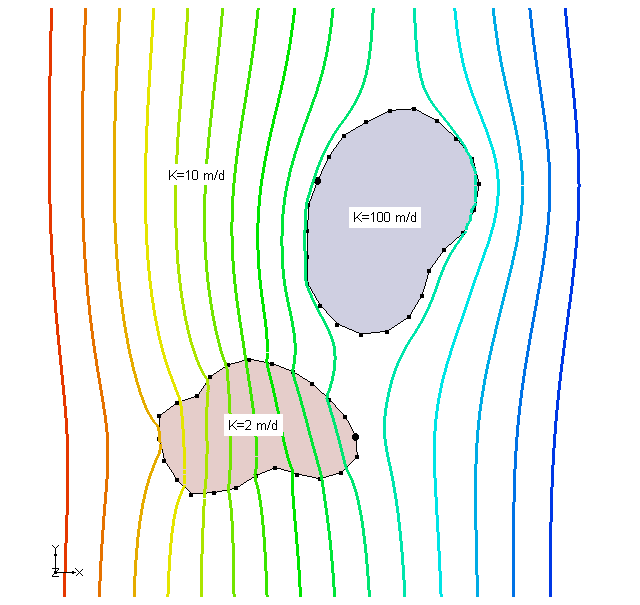
\includegraphics[width=6in,keepaspectratio,bb = 0 0 200 100, draft, type=eps]{figures/in0-polys.PNG}
	\end{centering}
	\caption{\label{cap:in0-polys}Potentiometric countours for two polygonal hydraulic conductivity inhomogeneities in a field of uniform flow. Flow is from left to right (red contours represent higher potentiometric heads). The domains are specified as follows: domain 0 (the outside) has $K=10\, m/d$; domain 1 has $K=100\, m/d$ and is shaded in blue; domain \#2 has $K=2\, m/d$ and is shaded in beige. No string specifications (\textsf{str} directive) were required.}
\end{figure}
\begin{figure}
	\begin{centering}
	%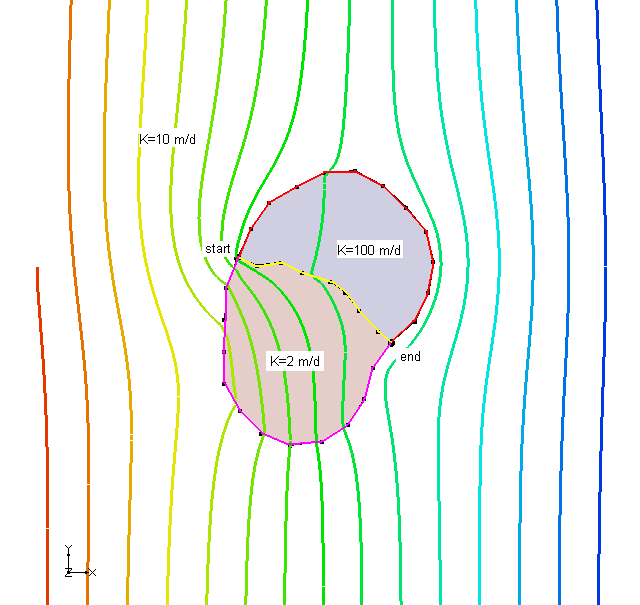
\includegraphics[width=6in,keepaspectratio,bb = 0 0 200 100, draft, type=eps]{figures/in0-strings.PNG}
	\end{centering}
	\caption{\label{cap:in0-strings}Potentiometric countours for two polygonal hydraulic conductivity inhomogeneities with a common boundary in a field of uniform flow. Flow from left to right (red contours represent higher heads). The domains are specified as follows: domain 0 (the outside) has $K=10\, m/d$; domain 1 has $K=100\, m/d$ and is shaded in blue; domain \#2 has $K=2\, m/d$ and is shaded in beige. Three strings are required; all share the same starting and ending points. The three strings are specified as follows: string 1 (red) has $left=0$, $right=1$; string 2 (yellow) has $left=1$; $right=2$; string 3 (purple) has $left=2$, $right=0$.}
\end{figure}
The following properties may be changed in ModAEM inhomogeneities:
\begin{itemize}
\item Hydraulic conductivity, $K$
\item Aquifer base elevation, $b$ 
\item Aquifer thickness, $H$
\item Aquifer effective porosity, $n$
\end{itemize}
In the case where base elevation and aquifer thickness are constant throughout the model domain, or when the flow is confined everywhere in the model, the equations solved by ModAEM for inhomogeneities are linear; only a few iterations are needed to achieve an accurate solution. In the case where the base elevation or aquifer thickness varies \emph{and} there are regions within the model where the flow is unconfined, the solution matrix contains coefficients that are dependent on the saturated thickness; additional iterations are required to achieve an accurate solution. For this reason, each sub-domain in the model has an additional parameter, the "initial average head''. The initial average head is the modeler's best estimate for the average head in the sub-domain. It is used to compute the saturated thickness during the first model iteration. Obviously, a good estimate for the initial average head helps the model stability.

\subsection{Specifying inhomogeneities}

As mentioned above, ModAEM allows for both closed polygonal inhomogeneities that do not share edges and for complex polygonal inhomogeneities that may have shared edges. ModAEM requires that the specification of inhomogeneities be done in two steps:
\begin{enumerate}
\item Defining the polygonal regions using the \textsf{dom} directive
\item Where necessary, defining the strings of elements that implement the boundaries using the \textsf{str} directive.
\end{enumerate}
Task (2) can be very complicated. Fortunately there are preprocessing tools such as GMS (EMS-I) and ArcInfo that provide an ``arc--node'' data representation to make it simpler. For many problems, inhomogeneities with common boundaries are unnecessary. Fortunately, ModAEM makes it easier to specify these (see below).

\paragraph{Usage:}
\begin{verbatim}
aqu ndomains nstrings base ...
  in0
    dom nvertices bot thick hyd-cond poro avg-head id
      (x1,y1)
      (x2,y2)
      ...
    dom ...
      ...
    str nvertices left right id
      (x1,y1)
      (x2,y2)
      ...
    str ...
      ...
  end
end
\end{verbatim}
As noted above, the maximum number of domains and strings to be used are specified in the \textsf{aqu} directive that begins the aquifer specification. The specification of inhomogeneities begins with the \textsf{in0} directive, which enters the inhomogeneity specification section of the ModAEM script file. Inside the IN0 section of the script, domains are specified first, then strings are defined that actually implement the boundaries\footnote{For problems without common boundaries, no string definitions are required; ModAEM automatically builds strings for closed domains.}.

\paragraph{Parameters for domain specification (directive \textsf{dom})}
\begin{description}
\item [{\texttt{nvertices}} (int)] The maximum number of vertices which may be used to delineate the boundary of the domain. $[-]$
\item [{\texttt{base}} (real)] The base elevation of the aquifer $[\mathrm{L}]$
\item [{\texttt{thickness}} (real)] The thickness of the aquifer $[\mathrm{L}]$
\item [{\texttt{conductivity}} (real)] The hydraulic conductivity (real) of the aquifer $[\mathrm{L/T}]$
\item [{\texttt{porosity}} (real)] Porosity of the aquifer as a fraction $[-]$
\item [{\texttt{initial-avg-head}} (real)] This is an estimate of the average head in the aquifer. It is used to pre--condition the solution when inhomogeneities in base elevation or thickness are encountered and the flow condition is unconfined. If you expect to be using inhomogeneities in base elevation or aquifer thickness, a good estimate of the initial average head will greatly speed the solution process. If you are not using inhomogeneities in base elevation or aquifer thickness, it is recommended that the value of $\mathtt{base+thickness}$ be provided. $[\mathrm{L}]$
$\{real\}$
As usual, flow may be confined and/or unconfined within the domain. If the flow is unconfined, additional iterations may be required for an accurate solution.
\item [{\texttt{id}} (int)] A unique identification number for the domain.
\end{description}

\paragraph{Specifying the vertices along the domain perimeter}
Following the \textsf{dom} directive, up to \texttt{nvertices} vertices may be provided, one vertex per line in the input file. Each vertex is a single complex coordinate. Each vertex is entered as a single complex coordinate, $\mathtt{(x_p, y_p)}$, where $p$ is the index of the vertex along the perimeter, $z_{p}=x_{p}+y_{p}$ $[\mathrm{L}]$


\paragraph{Parameters for string specification (directive \textsf{\textmd{str}})}

As mentioned above, ModAEM makes things easier for modelers who build input files by hand or from shapefiles that do not support an ``arc/node'' spatial data structure. If no common boundaries are to be specified, e.g. as in Figure \ref{cap:in0-polys}, the \textsf{str} directive should be omitted. ModAEM will automatically build closed strings of elements. The following describes the input format for inhomogeneity strings (please refer to Figure \ref{cap:in0-strings}).
\begin{description}
\item [{\texttt{nvertices}} (int)] The maximum number of vertices which may be used to delineate the string. $[-]$
\item [{\texttt{left}} (int)] The ID number of the polygon that is to the left of the string (see section \ref{sec:The-right--hand-rule}). $[-]$
\item [{\texttt{right}} (int)] The ID number of the polygon that is to the left of the string (see section \ref{sec:The-right--hand-rule}). $[-]$
\item [{\texttt{closed}} (logical)] Flag; if true, the string closes on itself, making a polygon. If false, the string is an open polyline. $[-]$
\item [{\texttt{id}} (int)] A unique identification number for the string. $[-]$
\end{description}

Once the aquifer is defined using module \textsf{AQU} (see Chapter \ref{cha:aqu-module}), additional boundary conditions are added to the model by superposition. This chapter describes the elements that are available in ModAEM. Currently, the following element modules are provided:

\begin{description}
\item [{Discharge--specified wells (\textsf{WL0})}] These are wells for which the pumping rate is known, for example, water supply wells or irrigation wells. This is the most commonly--used type of well; both pumping wells and injection wells are supported. These are analougous to wells created with the MODFLOW WEL package.

\item [{Head--specified wells (\textsf{WL1})}] These are wells for which the pumping rate is not \emph{a priori} known to the modeler. The best example is a dewatering well that turns on and off according to a water level measurement. For WL1 elements, the modeler provides the location and radius of the well, plus a location in the aquifer and a head value; ModAEM computes the pumping rate of the well\footnote{As will be discussed in Section \ref{sec:wl1-module}, \textsf{WL1} wells should not be confused with calibration targets or inverse models.}. These are somewhat analogous to MODFLOW constant--head cells.

\item [{Discharge--specified line sinks (\textsf{LS0})}] These are line segments that add or remove a specific amount of water along their length, where the modeler provides the amount of water to be added. Some examples of discharge--specified line sinks are infiltration galleries or rivers in arid climates that are typically dry, but infiltrate water at certain times of the year. These are analogous to a group of wells created with the MODFLOW WEL package.

\item [{Head--specified line sinks (\textsf{LS1})}] These are line segments that add or remove water along their lengths, but for which the pumping rate is not \emph{a priori} known to the modeler, and where there
is no ``entry resistance'', e.g a silty stream bed, between the line sink and the aa group ofquifer. \textsf{LS1} line sinks are often used to represent rivers in the far field when the modeler wishes to use an unbounded aquifer with a modeled far field (see Section \ref{sub:reference-flow-field}). These are somewhat analogous to a group of MODFLOW constant--head cells; they differ because in MODFLOW, constant head cells are specified as part of the BAS package, not as a separate component.

\item [{Resistance line sinks (\textsf{LS2})}] These are line segments that add or remove water along their lengths, but for which the pumping rate is not \emph{a priori} known to the modeler, and where an ``entry resistance'', e.g a silty stream bed, between the line sink and the aquifer is present. \textsf{LS2} line sinks are often used to represent surface waters or drains in the near field. \textsf{LS2} line sinks may be created as rivers (analogous to the MODFLOW RIV package), drains (analogous to the MODFLOW DRN package), or general--head boundaries (analogous to the MODFLOW GHB package). Streamflow routing may be performed for \textsf{LS2} elements (in a manner similar to the MODFLOW STR package), using the analysis module \textsf{RT0} (see Section \ref{sec:rt0-module}).

\item [{Horizontal no--flow boundaries (\textsf{HB0)}}] These are elements that create a linear no--flow condition within the active area of a ModAEM model. These may be used to model sheet pilings, slurry walls, faults, and other linear no--flow conditions that require an active aquifer domain on both sides of the line. This should not be used for bounded models or for ``islands'' in an aquifer domain; use the \textsf{BDY} elements included in module \textsf{AQU} (Section \ref{sub:bounded-aquifers}) for details. These are analougous to the MODFLOW HFB package.

\item [{Circular area--sinks (\textsf{PD0})}] These are elements that provide an areal infiltration or exfiltration rate over a circular sub--domain, using a circular ``pond'' function described by Strack (1989). The ``sink density'', or rate of infitration per unit of surface area, is specified by the modeler. These are typically used in example problems and for conceptual models, although they are convenient for representing circular irrigators. For most practical modeling applications, module \textsf{PD0} is superseded by the polygonal area--sink module \textsf{AS0} (Section \ref{sec:as0-module}).

\item [{Polygonal area--sinks (AS0)}] These are elements that provide an areal infiltration or exfiltration rate over a polygonal sub--domain. The ``sink density'', or rate of infitration per unit of surface area, is specified by the modeler. These are typically used as sources of areal recharge, e.g. from rainfall, or for infiltration galleries.
\end{description}
\newpage

\section{Discharge-specified wells (module \textsf{WL0})\label{sec:wl0-module}}

Module \textsf{WL0} creates discharge-specified wells. ModAEM processing enters module \textsf{WL0} in response to the \textsf{wl0} directive. 

\paragraph{Usage:}
\begin{verbatim}
    wl0 nwells
      (xw,yw) pumping-rate radius id 
  	     # Optional features follow if desired
         ppw ...
         eff ...
         dhd ...
         ddn ...
      (xw, yw) ...
      ...
    end
\end{verbatim}

\paragraph{Parameters for the \textsf{wl0} directive}

\begin{description}
  \item [\parameter{nwells}{int}] The maximum number of wells in the problem \units{-}
\end{description}

\paragraph{Specifying well elements}

The \textsf{wl0} directive is followed by one record for every well
in the model. If more than nwells well elements is provided, an ModAEM
will terminate and report the error. Each well record has the following
form:
\begin{verbatim}
    (xw,yw) pumping-rate radius id
\end{verbatim}

\paragraph{Parameters}

\begin{description}
\item [\parameter{(xw,yw)}{complex}] The coordinates of the center of the well. \units{L}
\item [\parameter{pumping-rate}{real}] The pumping rate of the well. The value is 
   positive if the element removes water from the aquifer, negative if it adds water 
   to the aquifer \footnote{Users who make use of ModAEM using the GMS preprocessor 
   will note that GMS makes use of the MODFLOW convention that abstraction of water 
   from the aquifer is negative, while injection is positive. Conversion to ModAEM's 
   convention is handled transparently by GMS.}. \units{L^3/T}
\item [\parameter{radius}{real}] The radius of the well. \units{L}
\item [\parameter{id}{int}] A unique identification number for the well. \units{-}
\end{description}

\paragraph{Optional \textsf{wl0} features} ModAEM offers several optional features for modeling discharge-specified wells. Two 


\newpage

\section{Head-specified wells (module WL1)\label{sec:wl1-module}}

Module WL1 creates head-specified wells. Head-specified wells should be used in cases where a well is to be used to maintain a particular water level at some location in the aquifer. The model computes the pumping rate for each head--specified well element that allows the model to match the specified head; these elements \emph{must not} be used for the purpose of calibrating the model to known heads. ModAEM processing enters module WL1 in response to the wl1 directive. 

\paragraph{Usage:}
\begin{verbatim}
    wl1 nwells
      (xw,yw) head (xc,yc) radius id
      ... 
    end
\end{verbatim}

\paragraph{Parameters}

\parameter{nwells}{int} The maximum number of wells in the problem \units{-}

\subsection{Specifying head--specified well elements}

The \textsf{wl1} directive is followed by one record for every well in the model. If more than nwells well elements is provided, an ModAEM will terminate and report the error. Each well record has the following form:
\begin{verbatim}
    (xw,yw) head (xc,yc) radius id
\end{verbatim}

\paragraph{Parameters}

\begin{description}
\item [\parameter{(xw,yw)}{complex}] The coordinates of the center of the well. \units{L}
\item [\parameter{head}{real}] The specified head at the control point. \units{L}
\item [\parameter{(xc,yc)}{complex}] The coordinates of the point where the head
condition is to be met. \units{L}
\item [\parameter{radius}{real}] The radius of the well. \units{L}
\item [\parameter{id}{integer}] A unique (integer) identification number for the
well. \units{-}
\end{description}
\newpage


\section{Discharge-specified line-sinks (module LS0) \label{sec:ls0-module}}

Module LS0 creates discharge-specified line-sinks. These are line
segments that add or remove a specific amount of water along their
length, where the modeler provides the amount of water to be added.
Some examples of discharge--specified line sinks are infiltration
galleries or rivers in arid climates that are typically dry, but infiltrate
water at certain times of the year. These are analogous to a group
of wells created with the MODFLOW WEL package.

\paragraph{Usage:}
\begin{verbatim}
    ls0 nstrings
      str npts id
        (x,y) strength 
        ...
      str ...
        ...
    end
\end{verbatim}

\paragraph{Parameters for the \textsf{ls0} directive}
\begin{description}
  \item [\parameter{nstrings}{integer}] The maximum number of discharge-specified
        line-sink strings in the problem. \units{-}
\end{description}
Following the \textsf{ls0} directive, the user provides strings of line sinks using the \textsf{str} directive. A string of line sinks is composed of a list of vertices. One 
line sink element is created for each pair of consecutive vertices.

\paragraph{Creating a string of elements}
\begin{verbatim}
    str npts id
      (x,y) strength
      ...
\end{verbatim}

\paragraph{Parameters}
\begin{description}
\item [\parameter{npts}{integer}] The maximum number of vertices in the line-sink
      string. \units{-}
\item [\parameter{id}{integer}] A unique identification number for the string. \units{-}
\end{description}

\paragraph{Specifying vertices for line--sink strings}
Following the \textsf{str} directive, two or more data records define
the vertices of the line--sink string. The parameters provided for
each vertex are as follows.
\begin{verbatim}
    (x,y) strength
\end{verbatim}
\begin{description}
\paragraph{Parameters}
\item [\parameter{(x,y)}{complex}] Coordinates of the vertex. \units{L}
\item [\parameter{strength}{real}] The sink density $\sigma$ of the line--sink
string at the vertex. The total volumetric infiltration or abstraction
along the line will be the value $(\sigma_{1}+\sigma_{2})\frac{L}{2}$
$[L^{3}/T]$ where $\sigma_{1}$ and $\sigma_{2}$ are the strengths
at consecutive vertices and $L$ is the distance between the vertices.
The sink density is defined as the total extraction rate of the line-sink
per unit length. The value is positive if the element removes water
from the aquifer, negative if it adds water to the aquifer
\footnote{Users who make use of ModAEM using the GMS preprocessor will note
that GMS makes use of the MODFLOW convention that abstraction of water
from the aquifer is negative, while injection is positive. Conversion
to ModAEM's convention is handled transparently by GMS.
}. \units{L^{2}/T}
\end{description}
\newpage


\section{Head-specified line-sinks (module \textsf{LS1})\label{sec:ls1-module}}

Module LS1 creates head--specified line--sink elements. These are line segments
that add or remove water along their lengths, but for which the pumping
rate is not \emph{a priori} known to the modeler, and where there
is no ``entry resistance'', e.g a silty stream bed, between the
line sink and the aquifer. LS1 line sinks are often used
to represent rivers in the far field when the modeler wishes to use
an unbounded aquifer with a modeled far field (see Section \ref{sub:reference-flow-field}).
These elements are somewhat analogous to a group of MODFLOW constant--head
cells; they differ because in MODFLOW, constant head cells are specified
as part of the aquifer, not as a separate element.

\paragraph{Usage:}
\begin{verbatim}
    ls1 nstrings
      str npts id
        (x,y) head 
          ...
      str ...
          ...
    end
\end{verbatim}

\paragraph{Parameters for the \textsf{ls1} directive}
\begin{description}
\item [\parameter{nstrings}{integer}] The maximum number of discharge-specified 
    line--sink strings in the problem. \units{-}
\end{description}
Following the \textsf{ls1} directive, the user provides strings
of line sinks using the \textsf{str} directive. A string of line sinks
is composed of a list of vertices. One line sink element is created
for each pair of consecutive vertices.

\paragraph{Creating a string of elements}
\begin{verbatim}
    str npts id
      (x,y) head
      ...
\end{verbatim}

\paragraph{Parameters for the \textsf{str} directive }
\begin{description}
\item [\parameter{npts}{integer}] The maximum number of vertices in the line-sink
string. \units{-}
\item [\parameter{id}{integer}] A unique identification number for the string. \units{-}
\end{description}

\paragraph{Specifying vertices for line--sink strings}
Following the \textsf{str} directive, two or more data records define
the vertices of the line--sink string. The parameters provided for
each vertex are as follows.
\begin{description}
\item [\parameter{(x,y)}{complex}] Coordinates of the vertex. \units{L}
\item [\parameter{head}{real}] The specified head at the center of the line-sink
   string. \units{L}
\end{description}
\newpage

\section{Line-sinks with entry resistance (module LS2)\label{sec:ls2-module}}

Module LS2 creates head-specified line-sinks. These are line segments
that add or remove water along their lengths, but for which the pumping
rate is not \emph{a priori} known to the modeler, and where an ``entry
resistance'', e.g a silty stream bed, between the line sink and the
aquifer is present. LS2 line sinks are often used to represent surface
waters or drains in the near field. LS2 line sinks may be created
as rivers (analogous to the MODFLOW RIV package), drains (analogous
to the MODFLOW DRN package), or general--head boundaries (analogous
to the MODFLOW GHB package). Streamflow routing may be performed for
LS2 elements (in a manner similar to the MODFLOW STR package), using
the analysis module RT0 (see Section \ref{sec:rt0-module}).

\paragraph{Usage:}
\begin{verbatim}
    ls2 nstrings
      str npts mode conductance id
        (x,y) head bottom
        ...
      str ...
        ...
    end
\end{verbatim}

\paragraph{Parameters for the \textsf{ls2} directive}
\begin{description}
\item [\parameter{nstrings}{integer}] The maximum number of discharge-specified 
   line--sink strings in the problem. \units{-}
\end{description}
Following the \textsf{ls2} directive, the user provides strings
of line sinks using the \textsf{str} directive. A string of line sinks
is composed of a list of vertices. One line sink element is created
for each pair of consecutive vertices.

\paragraph{Creating a string of elements}
\begin{verbatim}
    str npts mode conductance id
      (x,y) head bottom
      ...
\end{verbatim}

\paragraph{Parameters for the \textsf{str} directive }
\begin{description}
  \item [\parameter{npts}{integer}] The maximum number of vertices in the line-sink
    string. \units{-}
  \item [\parameter{id}{integer}] A unique identification number for the string. \units{-}
  \item [\parameter{mode}{integer}] Defines the behavior of the line sink. The value
    provided is an integer from the list below:
    \begin{description}
      \item [{\texttt{general-head boundary (0)}}] The boundary is always active,
        in a manner analogous with the MODFLOW GHB package.
      \item [{\texttt{river (1)}}] The line sink becomes a discharge--specified
        feature if the head in the aquifer falls below the bottom of the resistance
        layer (a ``percolating'' condition). In this case, the infiltration
        density is computed as $\sigma=c\times(h_{r}-h_{b})$ where $c$ is
        the conductance of the line sink (see below), $h_{r}$ is the specified
        stage in the river, and $h_{b}$is the elevation of the bottom of
        the resistance layer for this line sink. This is analogous to the
        MODFLOW RIV package.
      \item [{\texttt{drain (2)}}] The line sink will be removed from the solution
        with a sink density of zero when the head in the aquifer falls below
        the bottom of the drain. This is analogous to the MODFLOW DRN package.
    \end{description}
  \item [\parameter{conductance}{real}] The conductance for the line sink. The conductance
    is defined in a manner consistent with MODFLOW; for a river, the conductance
    is defined to be $c=w\times\frac{k_{c}}{t_{c}}\,[L/T]$, where $c$
    is the conductance, $w$ is the width of the stream, $k_{c}$ is the
    vertical hydraulic conductivity of the resistance layer, and $t_{c}$
    is the thickness of the resistance layer. \units{L/T}
  \item [\parameter{id}{integer}] A unique identification number for this string.
    \units{-} 
\end{description}

\paragraph{Specifying vertices for line--sink strings}
Following the \textsf{str} directive, two or more data records define
the vertices of the line--sink string. The parameters provided for
each vertex are as follows.
\begin{description}
  \item [\parameter{(x,y)}{complex}] Coordinates of the vertex. \units{L}
  \item [\parameter{head}{real}] The specified head at this vertex. The model 
    interpolates the head along the line segment. Since the head is specified at the
    center of the line segment, the average of the bottom elevation between
    adjacent vertices is used. \units{L}
  \item [\parameter{bottom}]{real} The elevation of the bottom of the resistance layer at
    this vertex. The model interpolates the bottom elevation along the
    line segment. Since the head is specified at the center of the line
    segment, the average of the bottom elevation between adjacent vertices
    is used. \units{L}
\end{description}
\newpage

\section{No--flow boundary walls (module HB0)\label{sec:hb0-module}}
Module HB0 creates no--flow boundary walls (e.g. sheet pilings or
slurry walls). These are elements that create a linear no--flow condition
within the active area of a ModAEM model. These may be used to model
sheet pilings, slurry walls, faults, and other linear no--flow conditions
that require an active aquifer domain on both sides of the line. This
should not be used for bounded models or for ``islands'' in an aquifer
domain; use the BDY elements included in module AQU (Section \ref{sub:bounded-aquifers})
for details. These are analogous to the MODFLOW HFB package.

\paragraph{Usage:}
\begin{verbatim}
    hb0 nstrings
      str npts id
        (x,y)
        ...
      str ...
        ...
    end
\end{verbatim}

\paragraph{Parameters for the \textsf{hb0} directive}
\begin{description}
\item [\parameter{nstrings}{integer}] The maximum number of no--flow strings in the
problem. \units{-}
\end{description}
Following the \textsf{hb0} directive, the user provides strings
of line sinks using the \textsf{str} directive. A no--flow string
is composed of a list of vertices. One line doublet element is created
for each pair of consecutive vertices.

\paragraph{Creating a string of elements}
\begin{verbatim}
    str npts id
      (x,y) strength
      ...
\end{verbatim}

\paragraph{Parameters for the str directive }
\begin{description}
  \item [\parameter{npts}{integer}] The maximum number of vertices in the line-sink
    string. \units{-}
  \item [\parameter{id}{integer}] A unique identification number for the string. 
    \units{-}
\end{description}

\paragraph{Specifying vertices for line--sink strings}
Following the \textsf{str} directive, two or more data records define
the vertices of the no--flow string. The parameters provided for each
vertex are as follows.
\begin{description}
  \item [\parameter{(x,y)}{complex}] Coordinates of the vertex. \units{L}
\end{description}

\section{Discharge-specified circular area-sinks (module PD0)\label{sec:pd0-module}}
Module PD0 creates discharge-specified circular area-sinks (colloquially
known as ponds). 

\paragraph{Usage:}
\begin{verbatim}
    pd0 nponds
      (xc,yc) strength radius id 
      ... 
    end
\end{verbatim}

\paragraph{Parameters for the \textsf{pd0} directive}
\begin{description}
\item [{\texttt{nwells}}] The maximum number of wells in the problem 
\end{description}

\paragraph{Specifying pond elements}
The \textsf{wl0} directive is followed by one record for every pond
in the model. If more than \texttt{nponds} elements are provided, ModAEM
will terminate and report the error. Each pond record has the following
parameters:
\begin{verbatim}
    (xc,yc) sink-density radius id\end{verbatim}
\begin{description}
  \item [\parameter{(xc,yc)}{complex}] The coordinates of the center of the pond. 
    \units{L}
  \item [\parameter{sink-density}{real}] The sink density of the pond. This is the
    value $\gamma=Q_{p}/A_{p}$, where $\gamma\,[L/T]$ is the sink density,
    $Q_{p}\,[L^{3}/T]$ is the total amount of water infiltrated or abstracted
    by the pond, and $A_{p}\,[L^{2}]$ is the area of the pond. The value
    is positive if the element removes water from the aquifer, negative
    if it adds water to the aquifer 
      \footnote{Users who make use of ModAEM using the GMS preprocessor will note
        that GMS makes use of the MODFLOW convention that abstraction of water
        from the aquifer is negative, while injection is positive. Conversion
        to ModAEM's convention is handled transparently by GMS.}
    \units{L/T}
  \item [\parameter{radius}{real}] The radius of the pond. \units{L}
  \item [\parameter{id}{real}] A unique identification number for the pond. \units{-}
\end{description}
\newpage

\section{Polygonal area-sinks (module AS0)\label{sec:as0-module}}
Module AS0 creates discharge-specified polygonal area--sink elements. These
are elements that provide an areal infiltration or exfiltration rate
over a polygonal sub--domain. The ``sink density'', or rate of infiltration
per unit of surface area, is specified by the modeler. These are typically
used as sources of areal recharge, e.g. from rainfall, or for infiltration
galleries. 
\paragraph{Usage:}
\begin{verbatim}
    as0 top/bottom nareas
      str npts strength id
        (x,y) 
        ...
      str ...
        ...
    end
\end{verbatim}
Please note: In versions of ModAEM prior to version 1.8, the ``bottom''
and ``nareas'' parameters were reversed in the AS0 input.

\paragraph{Parameters for the \textsf{as0} directive}
\begin{description}
  \item [\parameter{top/bottom}{integer}] An integer that specifies whether the area
    sinks are to be placed at the aquifer top (\texttt{\textbf{0}}) or
    bottom (\texttt{\textbf{1}}). \units{-}
  \item [\parameter{nareas}{integer}] The maximum number of discharge--specified 
    area--sink polygons in the problem. \units{-}
\end{description}
Following the \textsf{as0} directive, the user provides polygons using
the \textsf{str} directive. A polygon is composed of a list of vertices.
It is not necessary to duplicate the first vertex to close the polygon;
ModAEM automatically closes the polygon.

\paragraph{Creating an element}
\begin{verbatim}
    str npts sink-density id
      (x,y) 
      ...
\end{verbatim}

\paragraph{Parameters for the str directive }
\begin{description}
  \item [\parameter{npts}{integer}] The maximum number of vertices in the line-sink
    string. \units{-}
  \item [{\texttt{sink-density}}] The sink density of the area sink. This
    is the value $\gamma=Q_{p}/A_{p}$, where $\gamma\,[L/T]$ is the
    sink density, $Q_{p}\,[L^{3}/T]$ is the total amount of water infiltrated
    or abstracted by the element, and $A_{p}\,[L^{2}]$ is the area of
    the polygon. The value is positive if the element removes water from
    the aquifer, negative if it adds water to the aquifer.
      \footnote{Users who make use of ModAEM using the GMS preprocessor will note
        that GMS makes use of the MODFLOW convention that abstraction of water
        from the aquifer is negative, while injection is positive. Conversion
        to ModAEM's convention is handled transparently by GMS.}
    \units{L/T}
  \item [\parameter{id}{integer}] A unique identification number for the string. \units{-} \end{description}

\paragraph{Specifying vertices for polygons}
Following the \textsf{str} directive, three or more data records define
the vertices of the area--sink perimeter. The parameters provided
for each vertex are as follows.
\begin{description}
  \item[\parameter{(x,y)}{complex}] Coordinates of the vertex. \units{L}
\end{description}


\chapter{Processing Directives\label{cha:Processing-Directives} }

This chapter describes processing directives that control the solution
process and general imspection of values for ModAEM. Many of the directives
described here are most commonly used for program debugging, experimentation
and development of example problems. When computing results that are
to be used for analysis purposes (e.g. within GUI--based modeling
environments), the modules GRI (grid/contour generation), EXT (data
extraction), INQ (element results inquiry), and OBS (observation data)%
\footnote{Available in ModAEM-1.4.1 and later versions.%
}. See Chapter \ref{cha:Analysis-modules} for details about the analysis
modules.

Each of these directives is given outside the ``AEM section'' of
the ModAEM script. The general layout of the script is as follows,
with the processing directives marked in bold face.

\begin{verbatim}
    aem
      aqu...
        ref...
        bdy...
        in0...
          ...
        end
      end
      # Other elements go here
    end
    \textbf{\#processingdirectivesgohere}
    \textbf{sol...}
    \textbf{hea...}
    eod
\end{verbatim}
In nearly every case, the first processing directive issued should
be \texttt{\textbf{sol x}}, where \texttt{\textbf{x}} is the number
of iterations (if a solution is to be loaded, use \texttt{\textbf{sol
0}} to simply load the saved results file). After the solution is
complete, the other directives will be useful.


\paragraph{Processing directives for solving and reporting solution results }
\begin{description}
\item [{\texttt{SOL}}] Solves the model, based on the available input and
results from a previous solution loaded from disk%
\footnote{Available in ModAEM-1.4.1 and later versions.%
}.
\item [{\texttt{RPT}}] Generates a report of all solution information in
HTML format.
\end{description}

\paragraph{Processing directives that retrieve data from the model at specific
points}
\begin{description}
\item [{\texttt{HEA}}] Reports the head at some location in the model to
the error log file.
\item [{\texttt{POT}}] Reports the complex potential at some location in
the model to the error log file.
\item [{\texttt{DIS}}] Reports the discharge at some location in the model
to the error log file.
\item [{\texttt{VEL}}] Reports the velocity at some location in the model
to the error log file.
\item [{\texttt{RCH}}] Reports the net exfiltration rate at some location
in the model to the error log file.
\item [{\texttt{THK}}] Reports the saturated thickness at some location
in the model to the error log file.
\end{description}

\paragraph{Processing directives that compute numerical approximations for model
testing}
\begin{description}
\item [{\texttt{GRA}}] Reports the numerical gradient at some location
in the model to the error log file.
\item [{\texttt{LAP}}] Reports the numerical laplacian at some location
in the model to the error log file.
\end{description}

\paragraph{Processing directives that compute values for a line segment}
\begin{description}
\item [{\texttt{FLO}}] Reports the integrated flow across a line segment
in the model to the error log file.
\end{description}
The remainder of this chapter describes the general--purpose processing
directives in detail.\newpage


\section{Directive SOL -- solve the model }

After a model has been defined (using the AEM module input section),
it must be solved prior to performing any analyses. ModAEM uses an
iterative solution scheme -- at each iteration, the solution is improved
based on the previous iteration, including the incorporation of non--linear
elements such as resistance line sinks or inhomogeneity boundaries
in regions where the flow is unconfined.

\paragraph{Usage:}
\begin{verbatim}
    sol niter relaxation
\end{verbatim}

\paragraph{Parameters for the sol directive:}
\begin{description}
  \item [{niter}] The number of iterations to be performed. $\{integer\}$\\
  The number of iterations to be used depends strongly on the problem
  to be solved. The following list describes the issues that determine
  the number of iterations needed for model convergence. Note that this
  list is a rule--of--thumb; the modeler should look closely at the solution
  to ensure that it has fully converged.
  \begin{description}
    \item [{1--2iterations}] Simple models that are linear at all points
      in the domain. Typically, this means that the flow is confined everywhere
      and that no resistance line sinks that can be removed from solution
      (that is, ``river'' and ``drain'' line sinks) are present. These
      problems should give accurate solutions with only 1--2 iterations.
    \item [{3--8iterations}] More complex models that make use of ``river''
      and ``drain'' line sinks, or have large areas in the model domain
      in which the flow is unconfined, but where the aquifer base elevation
      and thickness are constant everywhere will typically converge in 8
      iterations or less.
    \item [{moreiterations}] Very complex models in which the aquifer base
      elevation and/or thickness varies and the flow is unconfined, or problems
      where baseflow routing is in use. These problems may require 10 or more 
    i  terations to achieve convergence.
  \end{description}
  \item [{relaxation}] The relaxation factor to be used. $\{integer\}$\\
    This parameter instructs ModAEM to relax the solution during iterations.
    If $relaxation=1$, then ModAEM applies all of the computed adjustments
    in the strength coefficients on each iteration. For $0<relaxation<1$,
    the value of $relaxation$ is multiplied by the strenght adjustments.
    In some very complex models, this reduces the ``stiffness'' of the
    solution algorithm and may reduce the possibility of oscillations
    during iterations. In nearly all cases, this parameter should be set
    to 1.0.
\end{description}

\subsection{Loading a previous solution}

In ModAEM-1.8 and later versions, the modeler has the option of loading a 
previous solution. This is an advantage for large complex models; the previous
solution may be loaded prior to post-processing and analysis, e.g. particle
tracking or computing grids of heads. The problem definition, i.e.
the aquifer definition and creation of all elements must be complete
prior to loading the results. 

Because the previous solution is loaded in response to the \textsf{sol}
directive a special version of the directive, \texttt{\textbf{sol
0}}, is provided. By issuing the \textsf{sol} directive with no iterations,
the previous solution will be loaded, and all of ModAEM's internal
data structures will be restored, but no addition solution step will
be performed. Whenever a previous solution is to be used, the \texttt{\textbf{sol
0}} directive should be the first directive in the ModAEM script after
the AEM section is complete.

\subsection{Saving a solution for future re--use}

If the modeler provides a name for a ``solution save file'' on line
3 of the ModAEM name file, ModAEM stores the solution there as the
final step in the ``post--solve'' procedure. No directives are required
in the ModAEM script file.

\section{Directive RPT -- report the solution in HTML format}

After the solution is complete (see directive \textsf{SOL} above), 

\section{Directives that compute analytic values at a single point}

The following procesing directives compute a value and report it in
a human--readable format to the run--time message file.

\subsection{\label{HEA_directive}HEA - report the modeled head}
Reports the potentiometric head at a specified point to the message
file and to the console. A solution must be present (see the \texttt{sol}
directive) prior to issuing this directive. 


\paragraph{Usage:}
\begin{verbatim}
hea(x,y)
\end{verbatim}

\paragraph{Parameters for the \textsf{hea} directive }
\begin{description}
\item [{\texttt{(x,y)}}] The desired location in the complex plane $x+iy$.
$\{complex\}$
\end{description}

\paragraph{Example:}

The head at the location $(100,100)$ is reported in response to the
following directive:
\begin{verbatim}
HEA(100.0,100.0)
\end{verbatim}

\subsection{\label{POT_directive}POT - report the modeled complex potential}

Reports the complex potential at a specified point to the message
file and to the console. The complex potential is defined as $\Omega=\Phi+i\Psi$,
where $\Phi$ is the discharge potential and $\Psi$ is the streamfunction%
\footnote{Note that the streamfunction does not exist for problems that include
recharge; the reported streamfunction value is not useful in regions
where a recharge element (see module AS0 or PD0) is present.%
}. A solution must be present (see the \texttt{sol} directive) prior
to issuing this directive.


\paragraph{Usage:}
\begin{verbatim}
pot(x,y)
\end{verbatim}

\paragraph{Parameters for the \textsf{pot} directive }
\begin{description}
\item [{\texttt{(x,y)}}] The desired location in the complex plane $x+iy$.
$\{complex\}$
\end{description}

\paragraph{Example}

The complex potential at the location $(100,100)$ is reported in
response to the following directive:
\begin{verbatim}
pot(100.0,100.0)
\end{verbatim}

\subsection{\label{DIS_directive}DIS - report the total aquifer discharge }

Reports the total aquifer discharge $Q_{x}+iQ_{y}$ at a specified
point to the message file and to the console. The total discharge
is a two-dimensional analogue for the specific discharge:
\[
Q_{i}=Q_{x}+iQ_{y}=\int_{z_{bot}}^{z_{top}}(q_{x}+iq_{y})dz
\]
 where $q_{x}(z)$ and $q_{y}(z)$ are the horizontal components of
the specific discharge $q_{i}=-k\partial_{i}H$ at the elevation $z$,
and $z_{top}$ and $z_{bot}$ are the elevations of the aquifer top
and bottom, respectively%
\footnote{Since ModAEM is a 2--D code, it does not explicitly compute the integral.
The value is computed analytically by differentiating the discharge
potential $\Phi$ at the coordinate $x+iy$. See e.g. Strack (1989)
or Haitjema (1995) for details. A detailed description of the formulation
of ModAEM will be included in a future version of this book.%
}. A solution must be present (see the \texttt{sol} directive) prior
to issing this directive. 


\paragraph{Usage:}
\begin{verbatim}
dis(x,y)
\end{verbatim}

\paragraph{Parameters for the \textsf{dis} directive }
\begin{description}
\item [{\texttt{(x,y)}}] The desired location in the complex plane $x+iy$.
$\{complex\}$
\end{description}

\paragraph{Example}

The complex discharge at the location $(100,100)$ is reported in
response to the following directive:
\begin{verbatim}
dis(100.0,100.0)
\end{verbatim}

\subsection{\label{VEL_directive}VEL - report the horizontal groundwater velocity }

Reports the horizontal aquifer velocity $v_{x}+iv_{y}$ at a specified
point to the message file and to the console. The velocity should
be interpreted as the \emph{vertically--averaged} velocity at the
point in question:
\[
\bar{v}_{i}=\bar{v}_{x}+i\bar{v}_{y}=\frac{Q_{i}}{hn_{e}}
\]
 where $\bar{v}_{x}(z)$ and $\bar{v}_{y}$ are the reported horizontal
components of the average velocity, $h$ is the saturated thickness,
and $n_{e}$ is the effective porosity. A solution must be present
(see the \texttt{sol} directive) prior to issing this directive. 


\paragraph{Usage:}
\begin{verbatim}
vel(x,y)
\end{verbatim}

\paragraph{Parameters for the \textsf{vel} directive }
\begin{description}
\item [{\texttt{(x,y)}}] The desired location in the complex plane $x+iy$.
$\{complex\}$
\end{description}

\paragraph{Example}

The average groundwater velocity at the location $(100,100)$ is reported
in response to the following directive:
\begin{verbatim}
vel(100.0,100.0)
\end{verbatim}

\subsection{\label{RCH_directive}RCH - report the net recharge rate}

Reports the net rate of areal recharge at a specified point to the
message file and to the console. The reported recharge rate has a
sign consistent with the ModAEM conventions as described in e.g.,
Sections\ref{sec:as0-module} and \ref{sec:pd0-module}. The reported
rate is negative if the net recharge rate injects water into the aquifer,
positive if water is removed. A solution must be present (see the
\texttt{sol} directive) prior to issuing this directive.


\paragraph{Usage:}
\begin{verbatim}
rch(x,y)
\end{verbatim}

\paragraph{Parameters for the \textsf{rch} directive }
\begin{description}
\item [{\texttt{(x,y)}}] The desired location in the complex plane $x+iy$.
$\{complex\}$
\end{description}

\paragraph{Example}

The net recharge rate (negative for recharge) at the location $(100,100)$
is reported in response to the following directive:
\begin{verbatim}
rch(100.0,100.0)
\end{verbatim}

\section{Directives that compute numerical approximations for testing}

Two directives are provided that approximately compute the gradient
in the potential and laplacian of the potential, for the purpose of
testing the analytic functions that underlie all ModAEM computations.


\subsection{GRA\label{GRA_directive} - report the modeled numerical gradient
in potential}

Reports the \emph{numerical} gradient in the discharge potential)
at a specified point to the message
file and console. This directive is commonly used in program debugging;
the numerical gradient should have approximately the same value as
the total discharge (see the \texttt{dis} directive in Section \ref{DIS_directive}).
A solution must be present (see the \texttt{sol} directive) prior
to issing this directive. 

The aproximate gradient $(\hat{q}_{x},\hat{q}_{y})$ is computed at
$(x,y)$, a point in the 2D plane, using a spacing $\delta$ provided
by the user. The calculations are performed according to the following
expression.

\begin{eqnarray*}
\hat{q}_{x} & = & \frac{1}{\delta}\left[\Phi(x+\delta,y)-\Phi(x-\delta,y)\right]\\
\hat{q}_{y} & = & \frac{1}{\delta}\left[\Phi(x,y+\delta)-\Phi(x,y-\delta)\right]
\end{eqnarray*}
in general, it is expected that a more accurate estimate of the gradient
is obtained by using a small value of $\delta$.


\paragraph{Usage:}
\begin{verbatim}
gra{[}z{]}delta
\end{verbatim}
Reports the numerical gradient in the potential at the complex coordinate,
$z=(x,y)$, using the spacing $\delta$. Note that in Fortran free-format
reads, the two parts of the complex coordinate are provided as $(x,y)$
pairs. 


\paragraph{Example:}

The numerical gradient at the coordinate $(100,100)$, using a spacing
of $1.0$ is reported in response to the following directive:
\begin{verbatim}
gra(100.0,100.0)1.0
\end{verbatim}

\section{Directives that compute a net analytic value for a line segment}

ModAEM provides a directive that is used to report model results along
a line segment. Future versions of ModAEM may include additional directives
for line segments.


\subsection{FLO\label{cmd:flo} - report the total flow across a path}

Directs ModAEM to report the total integrated groundwater flow across
a linear path connecting two specified points to the message
file (.err file) and console. The value is computed as

\[
Q(z_{1},z_{2})=\int_{z_{1}}^{z_{2}}Q_{n}ds
\]
where
\begin{description}
\item [{$z_{1}$and$z_{2}$}] are
the points at the end-points of the line segment, $z_{j}=x_{j}+iy_{j}$
\item [{$Q_{n}$}] is the discharge normal to the line segment
$z_{1}z_{2}$
\item [{$s$}] is the direction along the line segment $z_{1}z_{2}$
\end{description}
A solution must be present (see the \texttt{sol} directive) prior
to issing this directive. 


\paragraph{Usage:}
\begin{verbatim}
flo(x1,y1)(x2,y2)
\end{verbatim}
Reports the integrated groundwater flux across the line-segment connecting
$(x_{1},y_{1})$ and $(x_{2,}y_{2})$ in units of $L^{3}/T$. The
sign of the result is determined by the right-hand rule (Section \ref{sec:The-right--hand-rule}).


\paragraph{Example:}

The total integrated flux across the line segment containing $(50,50)$
and $(100,100)$ is reported in response to the directive
\begin{verbatim}
flo(50.0,50.0)(100.0,100.0)
\end{verbatim}

\section{Extracting model results in machine-readable format (module INQ)\label{sec:module-INQ}}

Module INQ provides the ability to extract results from the model
in a machine-readable format that is convenient for post-processing
tools and graphical user interface (GUI) programs.

This section needs to be completed


\chapter{Analysis modules\label{cha:Analysis-modules}}

\section{Generating grids of model results (module GRI)\ref{sec:gri-module}}

Module GRI provides a facility for the construction of grids (e.g.
for contour plotting) in a format compatible with SURFER\texttrademark,
Matlab\texttrademark, or other software packages. Within the grid
module, the window to be gridded must be specified, along with the
number of points on the long axis of the grid. 

5.7.1 Selecting the output file type (opt directive) The opt directive
instructs the grid module which type of output file to create. Usage:

opt grid-type The opt directive expects one parameter, as follows.
grid-type Choose surfer for an ASCII SURFER\texttrademark-compatible grid (with
the extension .grd) and matlab for

an ASCII MATLABTM-compatible grid (with the extension .m). If the
OPT directive is omitted, the grid-type will default to surfer.

Example To select a MatlabTM-compatible output file, issue the directive

opt matlab

5.7.2 Defining the grid window (win directive) Defines the window
to be gridded. Usage :

win (x1,y1) (x2,y2) The win directive expects the following parameters.
(x1,y1) The lower-left corner of the (rectangular) region to be gridded.
(x2,y2) The upper-right corner of the (rectangular) region to be gridded.

Example

win (-100.0,-100.0) (100.0,100.0)

sets the lower-left and upper-right corners of the window for the
GRI module at the coordinates \textbackslash{}Gamma \textbackslash{}Delta
\textbackslash{}Gamma 100\textbackslash{}Delta \textbackslash{}Delta
\textbackslash{}Gamma 100\textbackslash{}Theta and\textbackslash{}Gamma 

100\textbackslash{}Delta 100\textbackslash{}Theta , respectively.

5.7.3 Choosing the grid resolution (dim directive) Sets the number
of grid points along the long axis of the window. Usage:

dim npts The dim directive expects one parameter as follows. npts
The number of evenly-spaced points to compute along the long axis
of the rectangular grid region. Module GRI

will compute an appropriate number of points along the short axis
to ensure that the grid has regular spacing in both directions.

Example To make grid(s) with a resolution of 50 points along the long
axis, issue the directive

gri 50

5.7.4 Computing a grid and writing it to a file (directives hea, pot,
psi, q\_x, and q\_y) Once the grid type, grid region, and grid resolution
are specified (see the directives opt, dim, and win above), grid files
may be computed for a variety of model output values. Currently the
following directives are available:

HEA - Create a grid of heads Usage:

hea base-filename generates a grid of the potentiometric head f on
the file base-filename\_head.grd (or base-filename\_head.m)

POT - Create a grid of potentials Usage:

pot base-filename generates a grid of the discharge potential \textbackslash{}Phi
on the file base-filename\_potential.grd (or base-filename\_potential.m)

PSI - Create a grid of stream functions Usage:

psi base-filename generates a grid of the streamfunction \textbackslash{}Psi
on the file base-filename\_psi.grd (or base-filename\_psi.m)

Q\_X - Create a grid of discharges in the x-direction Usage:

q\_x base-filename generates a grid of the total aquifer discharge
in the x-direction potentiometric heads on the file base-filename\_qx.grd
(or base-filename\_qx.m)

Q\_Y - Create a grid of discharges in the y-direction Usage:

q\_y base-filename generates a grid of the total aquifer discharge
in the y-direction on the file base-filename\_qy.grd (or base-filename\_qy.m)


\section{Streamline tracing (module TR0)\label{sec:tr0-module}}

5.8 Module TR0 - Trace The TR0 directive instructs ModAEM to enter
the trace module, which is used to trace 2-D streamlines. The TR0
directive must have a matching END directive. Within the TR0 module,
the following directives are valid:

WIN - Set the tracing window. Default tuning parameters are derived
from the window size.

TUN - Set tuning parameters Sets tuning parameters for the tracing
algorithm. Usage:

TUN step prox frac small step The base step size prox The proximity
(in terms of the current step size) to boundary conditions for reducing
the step size frac The factor for step size reductions small Smallest
allowable step size

TIM - Specify maximum time allowed for particle tracing POI - Release
a single particle at the specified location LIN - Release particles
along a line N particles along a line

GRI - Release a grid of particles in the sub-window WL0 - Release
N particles in reverse from the well bore of a WL0 (discharge-specified
well) element. WL1 - Release N particles in reverse from the well
bore of a WL1 (head-specified well) element.


\chapter{Validation }

This chapter will describe the validation problems that ship with
the official ModAEM release.


\chapter{ModAEM Tools }

This chapter describes various preprocessing and postprocessing tools
that are either included in the ModAEM distribution or are available
from third-party vendors.


\bibliographystyle{plain}


\appendix
\chapter{Mathematical formulation of ModAEM elements}

Ugh...

\end{document}
